\documentclass[aspectratio=169,11pt]{beamer}

\usetheme{Madrid}
\usecolortheme{default}
\setbeamertemplate{navigation symbols}{}
\setbeamertemplate{footline}[frame number]

\usepackage{amsmath,amssymb}
\usepackage{graphicx}
\usepackage{tikz}
\usetikzlibrary{positioning,calc}
\usetikzlibrary{arrows.meta,decorations.pathmorphing}

\definecolor{RamRed}{RGB}{190,40,45}
\definecolor{RamBlue}{RGB}{30,90,180}
\definecolor{SoftGray}{RGB}{245,245,245}
\definecolor{DarkGray}{RGB}{70,70,70}
\definecolor{MapGreen}{RGB}{48,150,95}
\definecolor{MapGold}{RGB}{235,180,45}

\setbeamercolor{title}{fg=DarkGray}
\setbeamercolor{frametitle}{fg=white,bg=RamBlue}
\setbeamercolor{structure}{fg=RamBlue}

\tikzset{
  v/.style={circle,draw=black,fill=white,inner sep=1.8pt},
  edge/.style={draw=RamBlue,line width=1.25pt},
  topic/.style={draw=black!30,fill=SoftGray,rounded corners=5pt,inner sep=7pt,
    text width=5.8cm,minimum height=1.65cm,align=left},
}


\usepackage{booktabs}
\tikzset{dot/.style={circle,fill=black,inner sep=2pt}, lab/.style={circle,draw=black,fill=white,inner sep=2pt,minimum size=6mm,font=\small},selected/.style={draw=RamRed,line width=2pt}}

\newcommand{\Def}[2]{\begin{block}{#1}#2\end{block}}
\newcommand{\Thm}[2]{\begin{block}{#1}#2\end{block}}
\renewcommand{\Proof}[1]{\begin{block}{Proof}\normalsize #1\end{block}}
\newcommand{\Question}[1]{\begin{block}{Question}#1\end{block}}
\renewcommand{\Example}[1]{\begin{block}{Example}#1\end{block}}
\newcommand{\fall}[2]{#1^{\underline{#2}}}
\newcommand{\rise}[2]{#1^{\overline{#2}}}
\newcommand{\stir}[2]{\left\{\begin{matrix}#1\\#2\end{matrix}\right\}}
\newcommand{\cyc}[2]{\left[\begin{matrix}#1\\#2\end{matrix}\right]}
\newcommand{\eul}[2]{\left\langle\begin{matrix}#1\\#2\end{matrix}\right\rangle}
\newcommand{\coef}[2]{[#1^{#2}]}
\newcommand{\gap}{\par\medskip}

\title{Ramsey Theory}
\author{Jeremy Quastel}\date{}\begin{document}
\begin{frame}[plain]\begin{center}{\Huge\bfseries Ramsey Theory}\par\vspace{.25cm}{\Large Section 1.8}\par\vspace{.15cm}{\large Harris--Hirst--Mossinghoff, \emph{Combinatorics and Graph Theory}}\par\vspace{.1cm}\resizebox{!}{2.7cm}{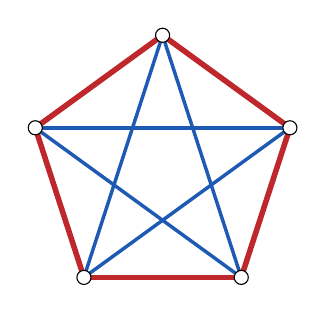
\begin{tikzpicture}[scale=1]
\coordinate (v1) at (0.000,1.700);
\coordinate (v2) at (-1.617,0.525);
\coordinate (v3) at (-0.999,-1.375);
\coordinate (v4) at (0.999,-1.375);
\coordinate (v5) at (1.617,0.525);
\draw[selected] (v1)--(v2);
\draw[edge] (v1)--(v3);
\draw[edge] (v1)--(v4);
\draw[selected] (v1)--(v5);
\draw[selected] (v2)--(v3);
\draw[edge] (v2)--(v4);
\draw[edge] (v2)--(v5);
\draw[selected] (v3)--(v4);
\draw[edge] (v3)--(v5);
\draw[selected] (v4)--(v5);
\node[v] at (v1) {};
\node[v] at (v2) {};
\node[v] at (v3) {};
\node[v] at (v4) {};
\node[v] at (v5) {};
\end{tikzpicture}}\par\vspace{.25cm}Jeremy Quastel\end{center}\end{frame}
\begin{frame}[plain]\large \begin{center}{\Huge\bfseries Today\textquotesingle s lecture}\par\vspace{.5cm}\end{center}\begin{columns}[c,onlytextwidth]\begin{column}{.48\textwidth}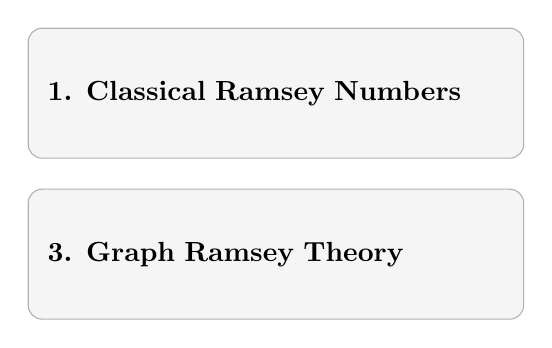
\begin{tikzpicture}\node[topic](a){\textbf{1. Classical Ramsey Numbers}};\node[topic,below=.38cm of a]{\textbf{3. Graph Ramsey Theory}};\end{tikzpicture}\end{column}\begin{column}{.48\textwidth}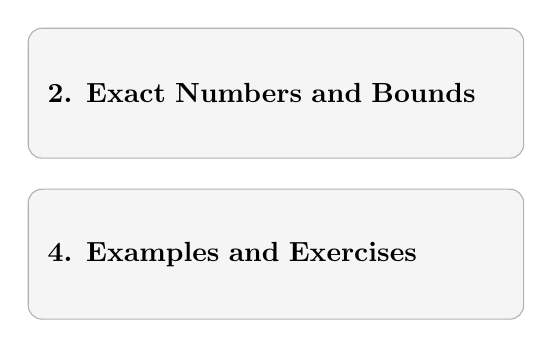
\begin{tikzpicture}\node[topic](a){\textbf{2. Exact Numbers and Bounds}};\node[topic,below=.38cm of a]{\textbf{4. Examples and Exercises}};\end{tikzpicture}\end{column}\end{columns}\end{frame}
\begin{frame}{A party problem}
\large
\Question{At a party of six people, must there be three mutual acquaintances or three mutual strangers?}
\gap Model people by vertices of $K_6$. Color an edge red for acquaintance and blue for stranger.
\gap We seek a triangle all of whose edges have the same color.
\end{frame}
\begin{frame}{Ramsey numbers}
\large
\Def{Classical Ramsey number}{For positive integers $p,q$, the Ramsey number $R(p,q)$ is the least $n$ such that every red--blue coloring of the edges of $K_n$ contains a red $K_p$ or a blue $K_q$.}
\gap Existence is part of Ramsey's theorem; it is not assumed in the definition.
\end{frame}
\begin{frame}{First observations}
\large
\[R(p,q)=R(q,p),\qquad R(1,q)=1,\qquad R(2,q)=q.\]
\Proof{Interchange the colors for symmetry. A single vertex is a copy of $K_1$. If there is no red edge in $K_q$, all edges are blue. Conversely, an all-blue $K_{q-1}$ has neither a red $K_2$ nor a blue $K_q$.}
\end{frame}
\begin{frame}{Why five people do not suffice}
\large
\begin{center}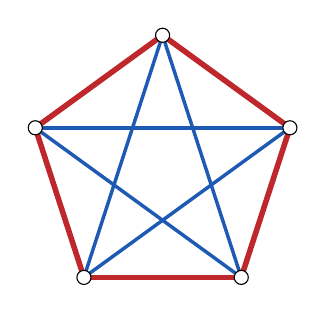
\begin{tikzpicture}[scale=1]
\coordinate (v1) at (0.000,1.700);
\coordinate (v2) at (-1.617,0.525);
\coordinate (v3) at (-0.999,-1.375);
\coordinate (v4) at (0.999,-1.375);
\coordinate (v5) at (1.617,0.525);
\draw[selected] (v1)--(v2);
\draw[edge] (v1)--(v3);
\draw[edge] (v1)--(v4);
\draw[selected] (v1)--(v5);
\draw[selected] (v2)--(v3);
\draw[edge] (v2)--(v4);
\draw[edge] (v2)--(v5);
\draw[selected] (v3)--(v4);
\draw[edge] (v3)--(v5);
\draw[selected] (v4)--(v5);
\node[v] at (v1) {};
\node[v] at (v2) {};
\node[v] at (v3) {};
\node[v] at (v4) {};
\node[v] at (v5) {};
\end{tikzpicture}\end{center}
\begin{center}The red edges form a $5$-cycle; so do the blue edges.\end{center}
\end{frame}
\begin{frame}{The lower bound for $R(3,3)$}
\large
\Proof{Neither color class in the displayed coloring of $K_5$ contains a triangle. Therefore
\[R(3,3)>5.\]}
\gap A lower bound requires \emph{one} coloring avoiding both targets. An upper bound must work for \emph{every} coloring.
\end{frame}
\begin{frame}{The upper bound: choose a vertex}
\large
\begin{center}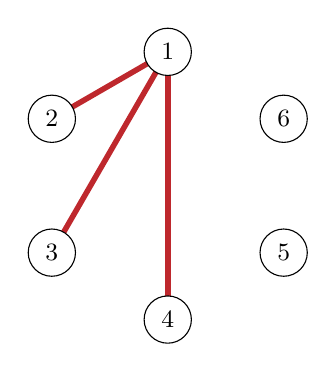
\begin{tikzpicture}[scale=1]
\coordinate (v1) at (0.000,1.700);
\coordinate (v2) at (-1.472,0.850);
\coordinate (v3) at (-1.472,-0.850);
\coordinate (v4) at (-0.000,-1.700);
\coordinate (v5) at (1.472,-0.850);
\coordinate (v6) at (1.472,0.850);
\draw[selected] (v1)--(v2);
\draw[selected] (v1)--(v3);
\draw[selected] (v1)--(v4);
\node[lab] at (v1) {1};
\node[lab] at (v2) {2};
\node[lab] at (v3) {3};
\node[lab] at (v4) {4};
\node[lab] at (v5) {5};
\node[lab] at (v6) {6};
\end{tikzpicture}\end{center}
\begin{center}At least three of the five edges at vertex $1$ have one color.\end{center}
\end{frame}
\begin{frame}{The upper bound: first possibility}
\large
\begin{center}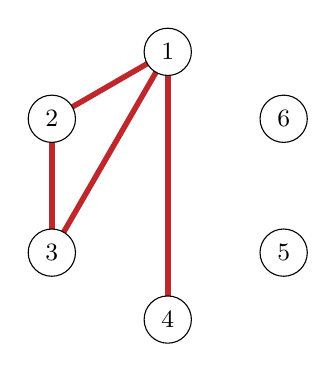
\begin{tikzpicture}[scale=1]
\coordinate (v1) at (0.000,1.700);
\coordinate (v2) at (-1.472,0.850);
\coordinate (v3) at (-1.472,-0.850);
\coordinate (v4) at (-0.000,-1.700);
\coordinate (v5) at (1.472,-0.850);
\coordinate (v6) at (1.472,0.850);
\draw[selected] (v1)--(v2);
\draw[selected] (v1)--(v3);
\draw[selected] (v1)--(v4);
\draw[selected] (v2)--(v3);
\node[lab] at (v1) {1};
\node[lab] at (v2) {2};
\node[lab] at (v3) {3};
\node[lab] at (v4) {4};
\node[lab] at (v5) {5};
\node[lab] at (v6) {6};
\end{tikzpicture}\end{center}
\begin{center}If one edge among the three neighbors is red, there is a red triangle.\end{center}
\end{frame}
\begin{frame}{The upper bound: second possibility}
\large
\begin{center}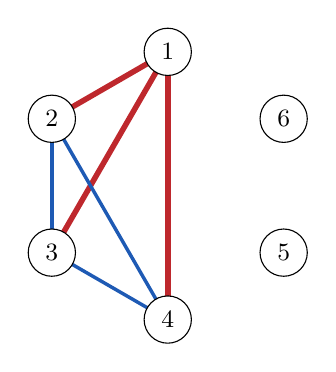
\begin{tikzpicture}[scale=1]
\coordinate (v1) at (0.000,1.700);
\coordinate (v2) at (-1.472,0.850);
\coordinate (v3) at (-1.472,-0.850);
\coordinate (v4) at (-0.000,-1.700);
\coordinate (v5) at (1.472,-0.850);
\coordinate (v6) at (1.472,0.850);
\draw[selected] (v1)--(v2);
\draw[selected] (v1)--(v3);
\draw[selected] (v1)--(v4);
\draw[edge] (v2)--(v3);
\draw[edge] (v3)--(v4);
\draw[edge] (v2)--(v4);
\node[lab] at (v1) {1};
\node[lab] at (v2) {2};
\node[lab] at (v3) {3};
\node[lab] at (v4) {4};
\node[lab] at (v5) {5};
\node[lab] at (v6) {6};
\end{tikzpicture}\end{center}
\begin{center}If none is red, the three neighbors form a blue triangle.\end{center}
\end{frame}
\begin{frame}{The first nontrivial Ramsey number}
\large
\Thm{Theorem}{\[R(3,3)=6.\]}
\Proof{The coloring of $K_5$ proves the lower bound $6$. The argument at an arbitrary vertex of $K_6$ proves the upper bound $6$.}
\end{frame}
\begin{frame}{The fundamental recurrence bound}
\large
\Thm{Theorem}{For $p,q\geq2$,
\[R(p,q)\leq R(p-1,q)+R(p,q-1).\]}
\gap This inequality proves that all classical Ramsey numbers are finite by induction on $p+q$.
\end{frame}
\begin{frame}{Proof of the recurrence bound}
\large
\Proof{Write $a=R(p-1,q)$ and $b=R(p,q-1)$, and color $K_{a+b}$. At a vertex $v$, let $A$ be its red neighbors and $B$ its blue neighbors.\gap Since $|A|+|B|=a+b-1$, either $|A|\geq a$ or $|B|\geq b$.\gap In the first case, $A$ contains a blue $K_q$ or a red $K_{p-1}$, which extends with $v$ to a red $K_p$. The second case follows by interchanging the colors.}
\end{frame}
\begin{frame}{A binomial upper bound}
\large
\Thm{Corollary}{For $p,q\geq2$,
\[R(p,q)\leq\binom{p+q-2}{p-1}.\]}
\Proof{The bound is exact on the boundary $p=2$ or $q=2$. Induct on $p+q$ and use Pascal's identity:
\[\binom{p+q-3}{p-2}+\binom{p+q-3}{p-1}=\binom{p+q-2}{p-1}.\]}
\end{frame}
\begin{frame}{Using the recurrence}
\large
\[R(3,4)\leq R(2,4)+R(3,3)=4+6=10.\]
\[R(4,4)\leq 2R(3,4)\leq20.\]
\gap These are upper bounds. The recurrence need not give the exact value.
\gap A parity argument sometimes improves the bound by $1$.
\end{frame}
\begin{frame}{The parity refinement}
\large
\Thm{Theorem}{If $a=R(p-1,q)$ and $b=R(p,q-1)$ are both even, then
\[R(p,q)\leq a+b-1.\]}
\Proof{Suppose a coloring of $K_{a+b-1}$ avoids both targets. At every vertex, red degree is at most $a-1$ and blue degree at most $b-1$. Their sum is $a+b-2$, so both bounds are attained.\gap The red graph has odd order $a+b-1$ and every degree $a-1$ is odd, contradicting the handshaking lemma.}
\end{frame}
\begin{frame}{The upper bound for $R(3,4)$}
\large
\[R(2,4)=4,\qquad R(3,3)=6.\]
Both numbers are even. Hence
\[R(3,4)\leq4+6-1=9.\]
\gap To prove equality, we need a coloring of $K_8$ with no red triangle and no blue $K_4$.
\end{frame}
\begin{frame}{A coloring on eight vertices}
\large
\begin{center}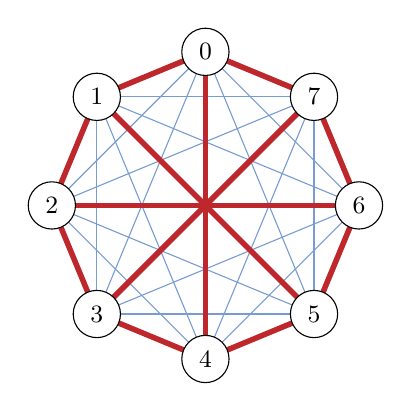
\begin{tikzpicture}[scale=1.3]
\foreach \i in {0,...,7}{\coordinate(v\i)at({90+45*\i}:1.5);}
\foreach \i in {0,...,7}{\foreach \j in {0,...,7}{\ifnum\i<\j\draw[RamBlue!60](v\i)--(v\j);\fi}}
\foreach \i in {0,...,7}{\pgfmathtruncatemacro{\j}{mod(\i+1,8)}\draw[selected](v\i)--(v\j);}
\foreach \i in {0,...,3}{\pgfmathtruncatemacro{\j}{\i+4}\draw[selected](v\i)--(v\j);}
\foreach \i in {0,...,7}{\node[lab]at(v\i){\i};}
\end{tikzpicture}\end{center}
\begin{center}Red: an $8$-cycle and the four opposite-vertex edges.\end{center}
\end{frame}
\begin{frame}{Why the coloring works}
\large
\Proof{The red graph has no triangle: the neighbors of a vertex are its two cyclic neighbors and its opposite vertex, and no two of these are adjacent in red.\gap A blue $K_4$ would be an independent set of size $4$ in the red graph. An independent $4$-set on an $8$-cycle must consist of alternate vertices. But either alternating set contains an opposite-vertex red edge.\gap Thus the coloring avoids both targets, and $R(3,4)\geq9$.}
\end{frame}
\begin{frame}{An exact value and a consequence}
\large
\Thm{Theorem}{\[R(3,4)=9.\]}
\gap Therefore
\[R(4,4)\leq R(3,4)+R(4,3)=18.\]
\gap Obtaining a matching lower bound requires a separate construction.
\end{frame}
\begin{frame}{The diagonal case}
\large
\[R(k,k)\leq\binom{2k-2}{k-1}<4^{k-1}\qquad(k\geq2).\]
\gap The proof gives a finite bound, but exact values become difficult quickly.
\Question{Can we also show that diagonal Ramsey numbers grow rapidly?}
\end{frame}
\begin{frame}{A random-coloring argument}
\large
\normalsize
Color each edge of $K_n$ independently red or blue, each with probability $1/2$. For a fixed set of $k\geq2$ vertices, the probability of a monochromatic clique is
\[2\left(\frac12\right)^{\binom{k}{2}}=2^{1-\binom{k}{2}}.\]
There are $\binom nk$ candidate vertex sets. By the union bound,
\[\Pr(\text{some monochromatic }K_k)\leq\binom nk2^{1-\binom{k}{2}}.\]
\end{frame}
\begin{frame}{A probabilistic lower bound}
\large
\Thm{Theorem}{If
\[\binom nk2^{1-\binom{k}{2}}<1,\]
then $R(k,k)>n$.}
\Proof{With positive probability, the random coloring has no monochromatic $K_k$. Therefore at least one such coloring exists.}
\gap An existence proof need not explicitly display the coloring.
\end{frame}
\begin{frame}{More than two colors}
\large
\Def{Multicolor Ramsey number}{$R(k_1,\ldots,k_r)$ is the least $n$ such that every $r$-coloring of $E(K_n)$ has a $K_{k_i}$ in color $i$ for some $i$.}
\gap The same neighborhood argument proves finiteness, using induction on the sum of the parameters.
\gap The two-color version is the main tool in this section.
\end{frame}
\begin{frame}{Graph Ramsey numbers}
\large
\Def{Graph Ramsey number}{For graphs $G,H$, let $R(G,H)$ be the least $n$ such that every red--blue coloring of $K_n$ has a red copy of $G$ or a blue copy of $H$.}
\gap Copies are subgraphs, not necessarily induced subgraphs.
\[R(G,H)\leq R(|V(G)|,|V(H)|).\]
\end{frame}
\begin{frame}{An immediate lower bound}
\large
\Thm{Observation}{For graphs $G,H$ of orders $m,n$,
\[R(G,H)\geq\min\{m,n\}.\]}
\gap A stronger construction uses the chromatic number of one graph and the size of a connected component of the other.
\end{frame}
\begin{frame}{A structural lower bound}
\large
\Thm{Theorem}{Let $c(G)$ be the largest order of a component of $G$. Then
\[R(G,H)\geq(c(G)-1)(\chi(H)-1)+1.\]}
\Proof{Take $\chi(H)-1$ disjoint red cliques, each of order $c(G)-1$, and color all edges between them blue. No red component is large enough to contain the largest component of $G$. The blue graph is $(\chi(H)-1)$-partite, so it cannot contain $H$.}
\end{frame}
\begin{frame}{Trees versus complete graphs}
\large
\Thm{Theorem}{For a tree $T_m$ on $m\geq2$ vertices and $n\geq2$,
\[R(T_m,K_n)=(m-1)(n-1)+1.\]}
\gap The structural lower bound gives the right-hand side. We prove the matching upper bound using chromatic number.
\end{frame}
\begin{frame}{A tree embedding lemma}
\large
\Thm{Lemma}{Every graph with minimum degree at least $m-1$ contains every tree of order $m$.}
\Proof{Induct on $m$. Delete a leaf $u$ of the tree, with neighbor $v$. By induction embed the remaining tree. The image of $v$ has at least $m-1$ neighbors, but at most $m-2$ other vertices are already used. An unused neighbor can receive $u$.}
\end{frame}
\begin{frame}{Trees versus complete graphs: upper bound}
\large
\Proof{Color $K_N$, where $N=(m-1)(n-1)+1$, and suppose there is no blue $K_n$. The red graph $F$ then has independence number at most $n-1$. Thus
\[\chi(F)\geq\left\lceil\frac{N}{n-1}\right\rceil\geq m.\]
Choose a subgraph minimal by vertex deletion with chromatic number at least $m$. Every vertex has degree at least $m-1$; otherwise an $(m-1)$-coloring after deletion extends back. The lemma gives a red $T_m$.}
\end{frame}
\begin{frame}{An example of the tree formula}
\large
\Example{Let $P_5$ be the path on five vertices. Then
\[R(P_5,K_3)=(5-1)(3-1)+1=9.\]}
\gap For the lower bound, use two red $K_4$'s with all edges between them blue.
\gap The theorem says every coloring of $K_9$ has a red $P_5$ or a blue triangle.
\end{frame}
\begin{frame}{Practice}
\large
\Question{Show that every red--blue coloring of $K_{10}$ has a red tree on four vertices of any prescribed shape, or a blue $K_4$.}
\gap What construction shows that $9$ vertices do not suffice?
\end{frame}
\begin{frame}{Practice: solution}
\large
\[R(T_4,K_4)=(4-1)(4-1)+1=10.\]
\gap For $K_9$, use three disjoint red triangles and make every edge between triangles blue.
\gap Red components have only three vertices, and a blue clique uses at most one vertex from each triangle.
\end{frame}
\begin{frame}{Summary}
\large
\begin{itemize}
\item Ramsey theory forces ordered substructures in sufficiently large colorings.
\item Lower bounds come from constructions; upper bounds apply to every coloring.
\item Neighborhood arguments give recurrence and binomial upper bounds.
\item Graph Ramsey numbers connect coloring, connectivity, and tree embeddings.
\end{itemize}
\end{frame}
\begin{frame}{Next time: Some Essential Counting Problems}\begin{center}{\Huge Some Essential Counting Problems}\end{center}\end{frame}
\end{document}